\documentclass[helvetica,openbib,logo,notitle,flagCMYK,totpages]{europecv}
\usepackage[T1]{fontenc}
\usepackage{graphicx}
\usepackage[a4paper,top=1.27cm,left=1cm,right=1cm,bottom=2cm]{geometry}
\usepackage[english]{babel}
\usepackage{url}
\usepackage{comment} 
\usepackage{emoji}
\usepackage{fontspec}
\setmainfont{Ubuntu}

% include background
\usepackage[scale=20,angle=-90,opacity=0.1]{background}
\backgroundsetup{contents={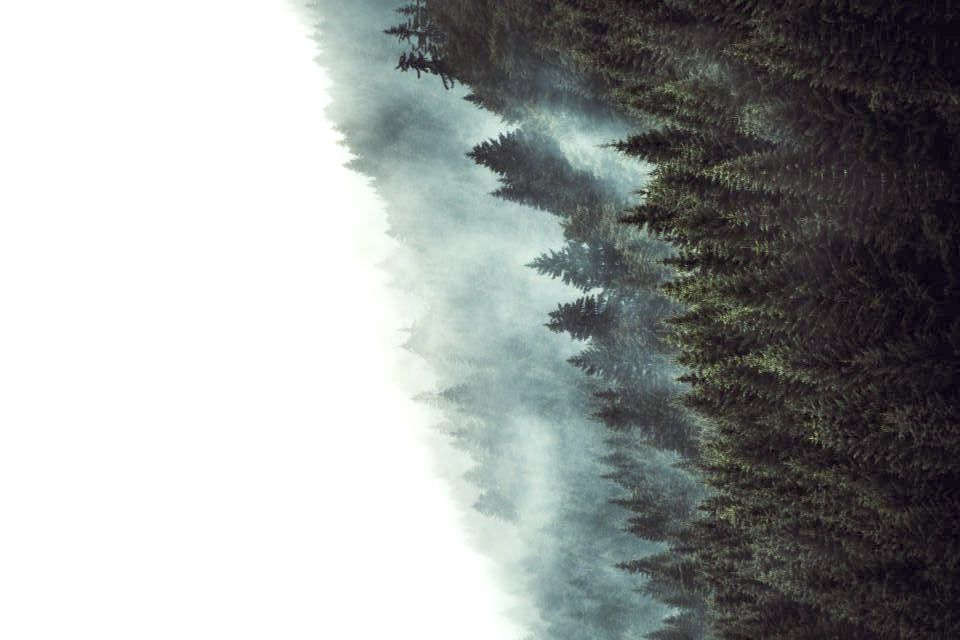
\includegraphics[width=.1\textwidth]{forest_1.jpeg}}}

\ecvname{Zignoli, Andrea}
\ecvfootername{Andrea Zignoli}
\ecvaddress{San Pietro In Cariano, Italy \emoji{flag-italy}}
% \ecvtelephone{mob. +39-340-811-XXXX}
\ecvhomepage{andreazignoli.github.io}
\ecvemail{Institutional: andrea.zignoli@unitn.it\newline 		
		Personal: andrea.zignoli@yahoo.it}
\ecvnationality{Italian \emoji{flag-italy}}
\ecvdateofbirth{Apr $24^{th}$, 1984}
\ecvgender{Male}
\ecvpicture[width=3cm]{profile_pic_1_1.png}
\ecvfootnote{For more information please email me.}

\begin{document}
\selectlanguage{english}

\begin{europecv}
\ecvpersonalinfo[5pt]
%%%%%%%%%%%%
%%%%%%%%%%%%
%%% foreword
\ecvsection{Current positions}
%% Athletica
\ecvitem{Date}{Since Apr 2020 \emoji{flag-united-states}}
\ecvitem{Part-time data scientist}{Athletica Inc. \newline
	Developing mathematical models of human performance for a virtual training platform. My activity mostly consists in supporting the app developers with my expertise in modelling the physiological and biomechanical response to exercise.  \newline
	Ref: Paul Laursen\newline}
%% Unitn
\ecvitem{Date}{Since Dec 2021 \emoji{flag-italy}}
\ecvitem{Teaching Fellow}{Department of Cellular, Computational and Integrative Biology - CIBIO, University of Trento, Trento, Italy.  \newline
Instructor for the 3-credit module on Modeling within the Technology and Innovation in Sports course in the Master’s program in Exercise Science and Human Movement
	Ref: Francesco Biral\newline}
%% Unitn
\ecvitem{Date}{Since Apr 2022 \emoji{flag-italy}}
\ecvitem{Fellow Researcher}{Department of Industrial Engineering, University of Trento, Trento, Italy.  \newline
	Ref: Francesco Biral\newline}
% SPEN
\ecvitem{Date}{Since Dec 2021 \emoji{flag-united-kingdom}}
\ecvitem{Associate Editor}{Sports Engineering Journal\newline
	Engagement with science and engineering communities. Work as Associate editor working alongside the other Editors and report to the Editor-in-Chief. \newline
	Ref: Thomas Allen\newline}

%%%%%%%%%%%%
\newpage
%%% work experience
\ecvsection{Research and work experience}
%%%%%%% Supersapiens
\ecvitem{Date}{Apr 2021 -- March 2024 \emoji{flag-united-states}}
\ecvitem{Full-time data scientist}{Supersapiens\newline
	Continuous glucose monitoring signal processing. My activities mostly consist in time series analyses (including anomaly detection and forecasting) and pattern recognition (sales, app usage data, etc.).  \newline
	Ref: Kristina Skroce\newline}
%%%%%%% visiting UQ
\ecvitem{Date}{Apr 2022 -- Nov 2022 \emoji{flag-australia}}
\ecvitem{Visiting researcher}{Exposed to the work done at the School of Human Movement and Nutrition Sciences, Faculty of Health and Behavioural Sciences, University of Queensland, Brisbane, Australia. \newline
	Ref: Jeff Coombes\newline}
%%%%%%% visiting SDU
\ecvitem{Date}{Oct 2021 -- Apr 2022 \emoji{flag-denmark}}
\ecvitem{Visiting researcher}{Exposed to the work done at the Research Unit Muscle Physiology and Biomechanics, Department of Sport and Biomechanics and the Center for Active and Healthy Aging, University of Southern Denmark, Odense, Denmark. \newline
	Ref: Paolo Caserotti\newline}
%%%%%%% post doc
\ecvitem{Date}{Dec 2020 -- Dec 2021 \emoji{flag-italy}}
\ecvitem{Postdoctoral researcher}{University of Trento, Department of Industrial Engineering.\newline
	The main goal of my activities is twofold: 1) to develop mathematical models (both first-principle and statistical/data-driven) for the sport technology industry and 2) to deploy such models on different platforms (from servers to microcontrollers) and deliver proofs of concepts of TRL 3 and 4. The outcome of my activities include scientific publications and state-of-the-art algorithms for sport performance analysis evaluation. \newline
	Ref: Francesco Biral\newline}
%%%%%%% post doc
\ecvitem{Date}{Nov 2019 -- Nov 2020 \emoji{flag-italy}}
\ecvitem{Postdoctoral researcher}{University of Trento \newline
	Department of Industrial Engineering\newline
	DDL-Meccatronica Project    \newline 
	Setup of "Deep Learning Lab" at the ProM Facility (TN, I). \newline
	Ref: Paolo Bosetti\newline}
%%%%%%% post doc
\ecvitem{Date}{Since Nov 2017 \emoji{flag-italy}}
\ecvitem{Postdoctoral researcher}{University of Trento \newline
	Department of Industrial Engineering\newline
	\emph{De Motu} Project    \newline 
	Designing physical and virtual models of the kinematic of the human knee. Research partners include: ProM Facility (TN, I), CeRiSM Research Centre (TN, I) and the MUSE Science Museum (TN, I). 
	\newline
	Ref: Francesco Biral\newline}
%%%%%%% visiting researcher
\ecvitem{Date}{Nov 2016 -- May 2017 \emoji{flag-japan}}
\ecvitem{Visiting researcher}{KAST \newline
	Kanagawa Academy of Science and Technology\newline
	KSP East, 3F, 3-2-1 Sakado, Takatsu-Ku, Kawasaki-Shi, Kanagawa 213-0012, Japan.\newline
	\emph{Development of Haptic Robots for Medicine, Rehabilitation, and Welfare} Project    \newline 
	Ref: Shimono Tomoyuki \newline}
%%%%%%% scholarship holder
\ecvitem{Date}{April 2016 -- July 2016 \emoji{flag-italy}}
\ecvitem{Scholarship holder}{CeRiSM Research Centre of Sport Mountain and Health, University of Verona, Department of Neurological and Movement Science, Verona (VR), Italy. \newline
	                         Human movement and physiological response to exercise data collection and analysis. Virtual modeling and optimal control algorithm application.    \newline 
	                         Ref: Federico Schena \newline}
%%%%%%% scholarship holder
\ecvitem{Date}{Jan -- Apr 2016 \emoji{flag-italy}}
\ecvitem{Collaboration}{University of Trento, Department of Industrial Engineering, Trento (TN), Italy.\newline 
	                    Development of virtual models of human bioenergetics and cycling biomechanics. \newline
	                    Ref: Francesco Biral \newline}
%%%%%%% PHD position
\ecvitem{Date}{Jan 2013 -- Dec 2015 \emoji{flag-italy}}
\ecvitem{PhD Student}{CeRiSM Research Centre of Sport Mountain and Health, University of Verona, Department of Neurological and Movement Science, Verona (VR), Italy. \newline Thesis title: \emph{Development of integrated tools for bio-mechanical analysis in sport performance: application to cycling}. The thesis aimed at developing bioenergetic and bio-mechanical models of cycling. The final goal was to apply the optimal-control approach in the attempt to replicate experimental data and predict the system behaviour by means of model simulation. \newline 
	Tutors: Barbara Pellegrini \& Francesco Biral \newline}
	
%%%%%%% abroad canada
\ecvitem{Date}{Mar -- Sept 2015 \emoji{flag-canada}}
\ecvitem{Visiting PhD student}{Human Performance Laboratory, Faculty of Kinesiology, University of Calgary, Calgary, AB, Canada.\newline 
	                                      Visiting student, research activity, working on musculoskeletal modeling of human lower limb, with focus on anatomical properties and muscle mechanics.    \newline
Ref: Walter Herzog \newline}
%%%%%%%%%%%%%%%%%%%%%%%%%%%%%%%%%%
	
%%%%%%% scholarship holder
\ecvitem{Date}{Apr -- Dec 2012 \emoji{flag-italy}}
\ecvitem{Scholarship holder}{CeRiSM Research Centre of Sport Mountain and Health, University of Verona, Department of Neurological and Movement Science, Rovereto (TN), Italy.\newline 
	                         Kinematic data collection and analysis, with focus on walking and running in fatigued conditions.    \newline 
	                         Ref: Federico Schena \newline}
	                         %%%%%%%%%%%%%%%%%%%%%%%%%%%%%%%%%%
%%%%%%% Arco plants
\ecvitem{Date}{Sept -- Dec 2011 \emoji{flag-italy}}
\ecvitem{Company internship}{ZF Padova S.r.l., Arco Plant, Arco (TN), Italy.\newline 
	                         BOM data analysis.    \newline 
	                         Ref: Daniele Dirignani (HR) \newline}
%%%%%%%%%%%%
%%%%%%% abroad UK
\ecvitem{Date}{Sept 2010 -- Mar 2011 \emoji{flag-united-kingdom}}
\ecvitem{Visiting Master student}{Integrity and Dynamics (\textsc{SID}) office, Research Group of the University of Nottingham, Nottingham, UK. \newline 
	                                      Developing different mathematical models of driver behaviour.   \newline
Ref: Atanas A. Popov \newline}
%%%%%%%%%%%%%%%%%%%%%%%%%%%%%%%%%%	                         
%%%%%%%%%%%%
%%%%%%%%%%%%
%%% education
\newpage
\ecvsection{Education and training}
%%%%%
\ecvitem{Place and Date}{University of Verona, Italy, 2013 -- 2015}
\ecvitem{PhD degree}{Movement Science and Physical Exercise (PhD). \newline 
	Thesis: \textit{Development of integrated tools for bio-mechanical analysis in sport performance: application to cycling}\newline
	Key Words: Mathematical modeling, optimal control, bioenergetics, biomechanics, human movement.\newline
	Tutors: Barbara Pellegrini  \& Francesco Biral\newline}
%%%%%
\ecvitem{Place and Date}{University of Trento, Italy, 2008 -- 2011}
\ecvitem{Master degree}{Mechatronic Engineering (M.Eng.), final grade: 105/110. \newline 
	            Thesis: \textit{Applications of Control Techniques to the Modeling of the Driver Behavior}\newline
	            Key Words: Model Predictive Control, mathematical modeling.\newline
	            Advisors: Prof. Francesco Biral  \& Prof. Atanas.A. Popov\newline}
%%%%%
\ecvitem{Place and Date}{University of Trento, Italy, 2003 -- 2008}
\ecvitem{Bachelor degree}{Industrial Engineering (B.Eng.), final grade: 92/110. \newline
	                      Thesis: \textit{Individuazione Statistica dell'Interfaccia di Cavitazione [Italian].}\newline
	                      Key Words: hydrodynamics, fluid Mechanics.\newline
	                      Advisor: Prof. Filippo Trivellato}
%%%%%%%%%%%%
%%%%%%%%%%%%
%%%%%%%%%%%%
\ecvsection{Personal skills and competences}

\ecvmothertongue[5pt]{Italian}
\ecvitem{\large Other language(s)}{English}
\ecvlanguageheader{(*)}
\ecvlanguage{English}{B2}{C1}{C1}{B2}{C1}
\ecvlanguagefooter[10pt]{(*)}


%%%%%%%%%%%%%%%%%%%%%%%%%%%%%%%%%%
%%%%%%%%%%%%%%%%%%%%%%%%%%%%%%%%%%
\ecvitem[10pt]{\large Technical skills and competences}{\textbf{Data acquisition}:\newline
	                                                   Basic level: Quark (CPET), k4-k5 metabolimeters, baropodometric pressure insoles
	                                                   \newline
	                                              	Advanced level: DELSYS Electromyography, QUALISYS/VICON Motion capture systems, SRM power meter, Lode Ergometer with Pedal Force Measurement System                      }
%%%%%%%%%%%%%%%%%%%%%%%%%%%%%%%%%%
%%%%%%%%%%%%%%%%%%%%%%%%%%%%%%%%%%
\ecvitem[10pt]{\large Computer skills and competences}{\textbf{Coding and software}: \newline 
Basic level: \LaTeX, OpenSim musculoskeletal modeling software, Linux OS, \textsc{C/C++} coding micro-processors (Arduino, Processing), RStudio (dplyr library) \newline  
Intermediate level: Maple, Microsoft Office, Microsoft Windows, Python programming language (Pandas, Scikit-learn), neural network development (by means of the neural network toolbox in the Matlab environment and the TensorFlow and Keras software libraries in Python environment), optimal control problem formulation and solution (by means of the software libraries GPOPS-II and PINS) \newline
Advanced level: Matlab}
%%%%%%%%%%%%%%%%%%%%%%%%%%%%%%%%%%
%%%%%%%%%%%%%%%%%%%%%%%%%%%%%%%%%%
\ecvitem[10pt]{\large Computer skills and competences}{\textbf{Signal processing}: \newline 
	Basic level: Pedal force measurements in cycling, force platform (anticipatory postural adjustments and centre of pressure trajectory), ski-pool with strain gauges (pooling forces in skiing), in-shoe pressure for comfort and cushioning, accelerometer and IMUs, GPS, odometers \newline  
	Intermediate level: Breath by breath pulmonary oxygen consumption, capillary blood lactate concentration, surface electromyography for muscle activation \newline
	Advanced level: Joint trajectory and body segment kinematics }
%%%%%%%%%%%%%%%%%%%%%%%%%%%%%%%%%%
%%%%%%%%%%%%%%%%%%%%%%%%%%%%%%%%%%
%%%%%%%%%%%%%%%%%%%%%%%%%%%%%%%%%%
%%%%%%%%%%%%%%%%%%%%%%%%%%%%%%%%%%
\newpage

\ecvsection{Statistics and data processing}

\ecvitem[10pt]{}{
$\bullet$ Classic statistics: normality check, mean difference (t-test), analysis of variance (ANOVA), repeated-measure ANOVA, multi-linear models (mainly conducted within the RStudio environment, i.e. with R language custom-written scripts).\newline
$\bullet$ Machine learning: principal component analysis, cluster analysis, random forest (mainly conducted within the Python environment, i.e. with custom-written scripts and scikit libraries).\newline
$\bullet$ Deep learning: long-short term memory (LSTM), recurrent neural networks (RNN), generative adversarial neural network (GAN), convolutional neural networks (CNN) (mainly conducted within the Python environment, i.e. with custom-written scripts and Keras-Tensorflow libraries).}
%%%%%%%%%%%%%%%%%%%%%%%%%%%%%%%%%%
%%%%%%%%%%%%%%%%%%%%%%%%%%%%%%%%%%
%%%%%%%%%%%%%%%%%%%%%%%%%%%%%%%%%%
\ecvsection{Fundings (ceased)}
\ecvitem[10pt]{}{
$\bullet$ ANTA Award, in collaboration with ECSS (European Congeress of Sport Science). The project consists in a research study titled “DARDAR project: Development (and deployment) of Algorithms to obtain Reliable stride-by-stride running kinematic Data in Real life conditions”. In collaboration with the Université de Franche Comté and Prof. Laurent Mourot. Total amount: 20000 €.
\newline
\newline
$\bullet$ ATHLETICA project: development of a web-based platform for training data processing and sport performance evaluation. Total amount: 9600 €.}
	                         
%%%%%%%%%%%%%%%%%%%%%%%%%%%%%%%%%%
%%%%%%%%%%%%%%%%%%%%%%%%%%%%%%%%%%
\ecvitem[10pt]{}{
$\bullet$ In collaboration with Selle Royal: study and development of a new testing protocol for high-quality cycling shoes. Total amount: 15000 €.
\newline
\newline
$\bullet$ Post-doctoral fellowship sponsored by the 
Fondazione Cassa di Risparmio di Trento e Rovereto (CARITRO) DDL-Meccatronica Project  to be developed at the \textit{deep learning lab} at the ProM Facility (TN, I). Total amount: 35000 €.	
\newline
\newline
$\bullet$ Restitution M5S 2019 for the development of a web-based application where data from cardiopulmonary exercise tests are used to train an automatic AI-diagnostic system. Total amount: 500 €.
\newline
\newline
$\bullet$ Starting Grant Young Researchers 2018 (internal call University of Trento) for a project proposal to be written together with Prof. Marcus Pandy at the University of Melbourne, Melbourne, Australia. Total amount: 5000 €.	
\newline
\newline
$\bullet$ Post-doctoral fellowship sponsored by the 
Fondazione Cassa di Risparmio di Trento e Rovereto (CARITRO) \textit{De Motu} project to be developed at the Department of Industrial Engineering of the University of Trento, Trento, Italy. Total amount: 25000 €.	
\newline
\newline
$\bullet$ International Cooperation grant 2015 for the project \textit{Modeling the Lower Limb of Cyclist} to be developed at the Human 
Performance Laboratory of the University of Calgary, AB, Canada. Total amount: 3000 €.	
\newline
\newline
$\bullet$ PhD student scholarship for three years between Jan 2013 and Dec 2015 at the University of Verona (Vr, I). Total amount: 60000 €.
\newline
\newline
$\bullet$ University of Trento scholarship for "The results achieved during the Master Course in Mechatronics Engineering". Total amount: 450 €. 
\newline
\newline
$\bullet$ Funded Erasmus scholarship for six months between Sept 2010 and Mar 2011 at the University of Nottingham (UK). Total amount: 3000 €.}
	                         
%%%%%%%%%%%%%%%%%%%%%%%%%%%%%%%%%%
%%%%%%%%%%%%%%%%%%%%%%%%%%%%%%%%%%


%%%%%%%%%%%%%%%%%%%%%%%%%%%%%%%%%%
%%%%%%%%%%%%
%%%%%%%%%%%%
%%%%%%%%%%%%
%%%%%%%%%%%%%%%%%%%%%%%%%%%%%%%%%%

\newpage
\ecvsection{Publications: journal papers (as leading author) LATEST}
% under development
% journals
%\ecvitem{}{\textbf{Journal paper}}
\ecvitem{}{
%%%%
%%%%
	\emph{AI-driven analysis of cardiopulmonary exercise tests to identify gas exchange and ventilatory thresholds}\newline 
	D. Keir, \textbf{A. Zignoli}, F.M. Maturana, D. Iannetta, J.M. Murias
    \newline 
    Sports Medicine, 2026. 
 \newline
	\newline
%%%%
	\emph{Assessing trajectories and bike handling abilities in road cycling
with global positioning system data}\newline 
	\textbf{A. Zignoli}
    \newline 
    Sensors, 2025. 
 \newline
	\newline
%%%%
%%%%
	\emph{Real-time assessment of exercising maximal mean power and speed in endurance sports: a Garmin connect IQ App}\newline 
	\textbf{A. Zignoli}, P. Whitehurst
    \newline 
    Sports Engineering - Technical note, 2025. 
 \newline
	\newline
%%%%
	\emph{Personalized nutrition and machine-learning: exploring the scope of continuous glucose monitoring in healthy individuals in uncontrolled settings}\newline 
	\textbf{A. Zignoli}, B. Martinez-Gonzalez, K. Skroce, D.J. Lipman, H.C. Zisser, A. Giorgi
    \newline 
    Int J Sport Nutr Exerc Metab., 2024. 
 \newline
	\newline
%%%%
%%%% 
	\emph{Personalized nutrition and machine-learning: exploring the scope of continuous glucose monitoring in healthy individuals in uncontrolled settings}\newline 
	\textbf{A. Zignoli}, K. Skroce, D.J. Lipman, H.C. Zisser
    \newline 
    Biomedical Signal Processing and Control, 2023. 
 \newline
	\newline
%%%%
%%%%
	\emph{Indoor running temporal variability for different running speeds, treadmill inclinations, and three different estimation strategies}\newline 
	\textbf{A. Zignoli}, A. Godin, L. Mourot
    \newline 
    PLOS-ONE, 2023. 
 \newline
	\newline
%%%%
%%%%
	\emph{Association between pre-exercise food ingestion timing and reactive hypoglycemia: insights from a large database of continuous glucose monitoring data}\newline 
	\textbf{A. Zignoli}, Federico Y. Fontana, K. Skroce, David J. Lipman, Felipe M. Maturana, Howard C. Zisser
    \newline 
    European Journal of Sport Science, 2023. 
 \newline
	\newline
%%%%
%%%% 
	\emph{How the Oxynet web applications are used to crowdsource and interpret cardiopulmonary exercising tests data}\newline 
	\textbf{A. Zignoli}, A. Fornasiero, F. Gilli, B. Pellegrini, F. Schena
    \newline 
    Biomedical Signal Processing and Control, 2023. 
 \newline
	\newline
%%%%
%%%% 
	\emph{Machine learning models for the automatic detection of exercise thresholds in cardiopulmonary exercising tests: from regression to generation to explanation}\newline 
	\textbf{A. Zignoli}
    \newline 
    Sensors, 2023. 
 \newline
	\newline
%%%%
%%%% 
}

\newpage
\ecvsection{Publications: journal papers (as leading author) CONT'D}
% under development
% journals
%\ecvitem{}{\textbf{Journal paper}}
\ecvitem{}{

%%%% 

	\emph{Insights in road cycling downhill performance using aerial drone footages and an ‘optimal’ reference trajectory}\newline 
	\textbf{A. Zignoli}, D. Fruet
    \newline 
    Sports Engineering - Technical note, 2022. 
 \newline
	\newline
%%%%
%%%% 
	\emph{An intelligent curve warning system for road cycling races}\newline 
	\textbf{A. Zignoli}
    \newline 
    Sports Engineering - Technical note, 2021. 
 \newline
	\newline
%%%%
%%%% 
	\emph{Assessment of bike handling during cycling individual time trials with a novel analytical technique adapted from motorcycle racing}\newline 
	\textbf{A. Zignoli}, F. Biral, A. Fornasiero, D. Sanders, T. Van Erp, M. Mateo-March, F.Y. Fontana, P. Artuso, P. Menaspà, M. Quod, A. Giorgi, P.B. Laursen
 \newline 
    European Journal of Sport Science, 2021. 
 \newline
	\newline
%%%%
%%%%
	\emph{Oxynet: a collective intelligence that detects ventilatory thresholds in cardiopulmonary exercise tests}\newline 
	\textbf{A. Zignoli}, A. Fornasiero, P. Rota, V. Muollo, L. A. Peyré-Tartaruga, D.A. Low, F.Y. Fontana, D. Besson, M. Pühringer, S. Ring-Dimitriou, L. Mourot
 \newline 
    European Journal of Sport Science, 2020. 
 \newline
	\newline
%%%%
%%%%
	\emph{Influence of corners and road conditions on cycling individual time trial performance and “optimal” pacing strategy: a simulation study}\newline 
	\textbf{A. Zignoli}
 \newline 
    Journal of Sports Engineering and Technology, 2020. 
 \newline
	\newline
%%%%
%%%%
	\emph{Estimating an individual's oxygen consumption during cycling exercise with a recurrent neural network trained from easy-to-obtain inputs}\newline 
	\textbf{A. Zignoli}, A. Fornasiero, M. Ragni, B. Pellegrini, F. Schena, F. Biral, P.B.Laursen
 \newline 
	PLOS-ONE, 2020. 
 \newline
	\newline
%%%%
%%%% 
	\emph{A new optimal control framework to predict realistic pacing and cornering strategies during cycling individual time trials}\newline 
	\textbf{A. Zignoli}, F. Biral \newline 
	Sports Engineering, 2020 \newline
	\newline
%%%% 
%%%% 
	\emph{State-of-the art concepts and future directions in modelling oxygen consumption and lactate concentration in cycling exercise}\newline 
	\textbf{A. Zignoli}, A. Fornasiero, E. Bertolazzi, B. Pellegrini, F. Schena, F. Biral, P.B. Laursen \newline 
	Sport Science for Health, 2019 \newline
	\newline
	%%%%%%
	%%%%%
	\emph{Expert-level classification of ventilatory thresholds from cardiopulmonary exercising test data with recurrent neural networks}\newline 
	\textbf{A. Zignoli}, A. Fornasiero, F. Stella, B. Pellegrini, F. Schena, F. Biral, P.B. Laursen \newline 
	European Journal of Sport Science, 2019 \newline
	\newline
	%%%%%%
	%%%%%
	\emph{Optimal control solution to the predictive dynamics of cycling}\newline 
	\textbf{A. Zignoli}, F. Biral, B. Pellegrini, A. Jinha, W. Herzog, F. Schena \newline 
	Sport Science for Health, 2017 \newline
	\newline
}
%%%%%%%%%%%%
%%%%%%%%%%%%
%%%%%%%%%%%%
\newpage 
\ecvsection{Publications: journal papers (as co-author) LATEST}
% under development
% journals
%\ecvitem{}{\textbf{Journal paper}}
\ecvitem{}{

        %%%%
        %%%%
    \emph{Quantitative ultrasound radiofrequency analysis for monitoring Parkinson's disease}\newline
	B. Bizet, M. Trinchi, F. Nardello, F. Bombieri, \textbf{A. Zignoli}, P. Zamparo, A. Monte
    \newline
	Neuroscience, 2026.
    \newline
	\newline
        %%%%
        %%%%
    \emph{Beyond Euglycemia: Case Studies Using Continuous Glucose Monitoring in
Elite Athletes Without Diabetes During Record Athletic Events}
	\newline 
	K. Skroce, Lauren V. Turner, \textbf{A. Zignoli}, David J. Lipman, Howard C. Zisser, Michael C. Riddell
    \newline
	\newline
    %%%%
    %%%%

        %%%%
        %%%%
    \emph{Continuous glucose monitoring–derived glucose metrics over time in physically active adults without diabetes using a commercial Continuous Glucose Monitoring application}
	\newline 
	K. Skroce, \textbf{A. Zignoli}, Lauren V. Turner, David J. Lipman, Michael C. Riddell, Howard C. Zisser
    \newline
	\newline
    %%%%
    %%%%
    
    
    %%%%
        %%%%
    \emph{Topical collection: Fluid Dynamics in Sports}
	\newline 
	F. Malizia, \textbf{A. Zignoli}, · K.E. Teigen Giljarhus
    \newline 
	Sports Engineering, 2025. 
    \newline
	\newline
    %%%%
    %%%%
    %%%%
    \emph{Continuous Glucose Monitoring Profiles in Elite-Level Professional European Football Players}
	\newline 
	K. Skroce, \textbf{A. Zignoli}, N. Mihic, D.J. Lipman, L.V. Turner, M.C. Riddell, and H.C. Zisser
    \newline 
	Journal of Diabetes Science and Technology, 2025. 
    \newline
	\newline
    %%%%
    %%%%
    %%%%
    %%%%
    \emph{Moderate heart rate-matched hypoxic exercise: autonomic and cardiovascular responses to different degrees of hypoxic stress}
	\newline 
	A. Fornasiero, A.G. Represas, \textbf{A. Zignoli}, F. Stella, M. Rakobowchuk, L. Mourot
    \newline 
	European Journal of Applied Physiology , 2025. 
    \newline
	\newline
    %%%%
    %%%%
}

%%%%%%%%%%%%%%%%%%%%%%%%%%%%%%%%%%
%%%%%%%%%%%%%%%%%%%%%%%%%%%%%%%%%%
\newpage 
\ecvsection{Publications: journal papers (as co-author) CONT'D}
% under development
% journals
%\ecvitem{}{\textbf{Journal paper}}
\ecvitem{}{
    %%%%
    %%%%
    \emph{Assessing Energy Availability and Glucose Dynamics in Adolescent
Cyclists: Implications for Nutritional Interventions during Competitive Season}
	\newline 
	M. Tarocchi, A. Pellegrino, K. Skroce, \textbf{A. Zignoli}, L.C. Cavadini, C. Bodini, G. Pagliai, L.
Toncelli, L. Stefani, S. Vanni, M. Boddi, A. Modesti,
P.A. Modesti 
    \newline 
	Nutrients, 2024. 
    \newline
	\newline
    %%%%
    %%%%
%%%%
%%%%
    \emph{Design and development of a feedback system for automatic treadmill speed adaptation}
	\newline 
	D. Fruet, \textbf{A. Zignoli}, R. Modena, B. Pellegrini, L. Gastaldi, L. Bortolan
    \newline 
	Proceedings of the Institution of Mechanical Engineers Part P Journal of Sports Engineering and Technology, 2024. 
    \newline
	\newline
    %%%%
    %%%%
    \emph{Real World Interstitial Glucose Profiles of a Large Cohort of Physically Active Men and Women}
	\newline 
	K. Skroce, \textbf{A. Zignoli}, F.Y. Fontana,F.M. Maturana, D. Lipman, A. Tryfonos, M.C. Riddell, H.C. Zisser
    \newline 
	Sensors, 2024. 
    \newline
	\newline
    %%%%
    %%%%
    \emph{The effects of a 6-hour ultra-endurance run on postexercise parasympathetic reactivation responses}
	\newline 
	A. Fornasiero, \textbf{A. Zignoli}, B. Pellegrini, F. Schena, G. Doucende, L. Mourot
    \newline 
	The Journal of sports medicine and physical fitness, 2023. 
    \newline
	\newline
    %%%%
    	\emph{Eager to set a record in a vertical race? Test your VO2max first!}
	\newline 
	A. Fornasiero, A. Savoldelli, \textbf{A. Zignoli}, A. Callovini, M. Decet, L. Bortolan, F. Schena, B. Pellegrini
    \newline 
	Journal of Sports Sciences, 2023. 
    \newline
	\newline
	%%%%
    %%%%
	\emph{Knee flexor and extensor torque ratio in elderly men and women with and without obesity: a cross-sectional study}
	\newline 
	V. Muollo, \textbf{A. Zignoli}, L. Ghiotto, C. Milanese, M. Zamboni, F. Schena, A.P. Rossi
    \newline 
	Aging Clinical and Experimental Research, 2021. 
    \newline
	\newline
	%%%%
    %%%%
	\emph{Response to Chaen and Trapellieni re: "Shortening Work-Rest Durations Reduces Physiological and Perceptual Load During Uphill Walking in Simulated Cold High-Altitude Conditions," by Fornasiero et al}
	\newline 
	A. Fornasiero, \textbf{A. Zignoli}, M. Rakobowchuk, F. Stella, S. Skafidas, A. Savoldelli, B. Pellegrini, F. Schena, L. Mourot
    \newline 
	High Altitude Medicine \& Biology, 2021. 
    \newline
	\newline
	%%%%
    %%%%
	\emph{Post-exercise cardiac autonomic and cardiovascular responses to heart rate matched and work rate matched hypoxic exercise}
	\newline 
	A. Fornasiero, \textbf{A. Zignoli}, M. Rakobowchuk, F. Stella, S. Skafidas, A. Savoldelli, B. Pellegrini, F. Schena, L. Mourot
    \newline 
	European Journal of Applied Physiology, 2021. 
    \newline
	\newline
	%%%%
	%%%% 
	\emph{Full characterisation of knee extensors’ function in ageing: effect of sex and obesity}
	\newline 
	V. Muollo, A. Rossi, \textbf{A. Zignoli}, M. Teso, C. Milanese, V. Cavedon, M. Zamboni, F. Schena, C. Capelli, S. Pogliaghi
    \newline 
	International Journal of Obesity, 2020. 
    \newline
	\newline
	%%%%
    %%%%
	\emph{Muscle and tendon stiffness and belly gearing positively correlate with rate of torque development during explosive fixed end contractions}
	\newline 
	A. Monte, \textbf{A. Zignoli}
    \newline 
	Journal of Biomechanics, 2020. 
    \newline
	\newline
	%%%%
}
	       % posters
%%%%%%%%%%%%%%%%%%%%%%%%%%%%%%%%%%
% \ecvitem{}{\textbf{Contribution in congress}}
\ecvsection{Publications: journal papers (as co-author) CONT'D}
\ecvitem{}{
%%%
		%%%% 
	\emph{Post-exercise hypotension and reduced cardiac baroreflex after
    half-marathon run: in men, but not in women}
    \newline 
	L. Mourot, A. Fornasiero, M. Rakobowchuk, L. Isacco, A. Brighenti, F. Stella, \textbf{A. Zignoli}, B. Pellegrini, C. Tarperi, F. Schena
    \newline 
	International Journal of Environmental Research and Public Health, 2020. 
    \newline
	\newline
	%%%%
		%%%% 
%%%%
	\emph{Shortening Work-Rest Durations Reduces Physiological and Perceptual Load During Uphill Walking in Simulated Cold High-Altitude Conditions}
	\newline 
	A. Fornasiero, A. Savoldelli, F. Stella, A. Callovini, L. Bortolan, \textbf{A. Zignoli}, D. Low, L. Mourot, F. Schena, B. Pellegrini
    \newline 
	High Altitude Medicine \& Biology, 2020. 
    \newline
        \newline
    %%%%
\emph{Similar cardiovascular and autonomic responses in trained type 1 diabetes mellitus and healthy participants in response to half marathon}
    \newline 
	L. Mourot, A. Fornasiero, M. Rakobowchuk, S. Skafidas, A. Brighenti, F. Stella, \textbf{A. Zignoli}, A. Savoldelli, B. Pellegrini, E. Danese, G. Lippi, C. Tarperi, F. Schena
    \newline 
	Diabetes Research and Clinical Practice, 2019. 
    \newline
	\newline
	%%%%
		%%%% 
	\emph{Cardiac autonomic and physiological responses to moderate-intensity exercise in hypoxia}
	\newline 
	A. Fornasiero, S. Skafidas, S. Stella, \textbf{A. Zignoli}, S. Aldo, M. Rakobowchuk, B. Pellegrini, F. Schena, L. Mourot
    \newline 
	International Journal of Sport Medicine, 2019. 
    \newline
	\newline
	%%%% 
	%%%% 
	\emph{Delayed parasympathetic reactivation and sympathetic withdrawal following maximal cardiopulmonary exercise testing (CPET) in hypoxia} 
	\newline 
	A. Fornasiero, A. Savoldelli, S. Skafidas, F. Stella, L. Bortolan, G. Boccia, \textbf{A. Zignoli}, F. Schena, L. Mourot, B. Pellegrini 
	\newline 
			European Journal of Applied Physiology, 2018
	\newline
	\newline
	% 2 %%%%%%%%%
	%%%% 
	\emph{Physiological factors associated with ski-mountaineering vertical race performance}
	\newline 
	A. Fornasiero, A. Savoldelli, G. Boccia, \textbf{A. Zignoli}, L. Bortolan, F. Schena, B. Pellegrini 
	\newline 
	Sport Science for Health, 2017  
	\newline
	\newline
	%%%% 
%%%%%%%%%%
	\emph{An Extreme Mountain Ultra-Marathon Decreases the Cost of 	Uphill Walking and Running} 
	\newline 
	Vernillo G., Savoldelli A., Skafidas S., \textbf{Zignoli A.}, La Torre A., Pellegrini B., Giardini G., Trabucchi P., Millet G.P. and Schena F.
	\newline 
	Frontiers in Physiology, 2016
	\newline
	\newline
	% 2 %%%%%%%%%
	\emph{Energy Cost and Kinematics of Level, Uphill and Downhill Running: Fatigue-Induced Changes After a Mountain Ultramarathon} 
	\newline 
   G. Vernillo, A. Savoldelli, \textbf{A. Zignoli}, S. Skafidas, A. Fornasiero, A. La Torre, L. Bortolan, B. Pellegrini, F. Schena
   \newline 
   Journal of Sports Science, 2015
   \newline
   \newline
   % 3 %%%%%%%%%
   \emph{Influence of the world's most challenging mountain ultra-marathon on energy cost and running mechanics} \newline
   Vernillo G., Savoldelli A., \textbf{Zignoli A.}, Trabucchi P., Pellegrini B., Millet G.P., Schena F. \newline
   European Journal of Applied Physiology, 2014
   \newline
}
% posters
%%%%%%%%%%%%%%%%%%%%%%%%%%%%%%%%%%
% \ecvitem{}{\textbf{Contribution in congress}}
\ecvsection{Pubblications: peer-reviewed conference proceedings}
\ecvitem{}{
\emph{Continuous Glucose Monitoring of Non-Diabetic Professional Cyclists during a Training Camp}\newline
	       A. Giorgi, B. Martinez-Gonzalez, M. Vicini, \textbf{A. Zignoli}, K. Skroce \newline
	       Science \& Science Conference, 2023
	       \newline
	       \newline
		%%%%%%%%
	       \emph{Automatic Generation of Realistic Cardiopulmonary Exercise Test Data With a Conditional Generative Adversarial Neural Network}\newline
	       \textbf{A. Zignoli}, D. Fruet \newline
	       Workshop on Sport, Technology and Research - IEEE, 2022
	       \newline
	       \newline
   		%%%%%%%%
	       \emph{Developing a Testing Protocol to Assess the Mechanical Properties of High-Level Cycling Shoes}\newline
	       D. Fruet, \textbf{A. Zignoli}, V. Fontanari, F. Biral, S. Raghavendra, M. Pezzato, E. Saeter \newline
	       Workshop on Sport, Technology and Research - IEEE, 2022
	       \newline
	       \newline
  		%%%%%%%%
	       \emph{Estimating Running Kinematics Variability With an IMU Sensor Placed on the Runner's Thorax}\newline
	       \textbf{A. Zignoli}, L. Mourot, D. Fruet \newline
	       Workshop on Sport, Technology and Research - IEEE, 2022
	       \newline
	       \newline
 		%%%%%%%%
	       \emph{Biomechanical Analysis and Modeling of Anterior Cruciate Ligament Rupture Conditions: Focus on Female Soccer Players}\newline
	       \textbf{A. Zignoli}, L. Tonelli, D. Fruet, F. Biral, V. Fontanari \newline
	       Workshop on Sport, Technology and Research - IEEE, 2022
	       \newline
	       \newline
		%%%%%%%%
	       \emph{Real-time cross-dataset quality production Assessment in industrial laser cutting machines}\newline
	       N. Peghini, \textbf{A. Zignoli}, D. Gandolfi, P. Rota, P. Bosetti \newline
	       1st International Workshop on Industrial Machine Learning - ICPR, 2020
	       \newline
	       \newline
		%%%%%%%%
	       \emph{Including a musculoskeletal model in the control loop of an assistive robot for the design of optimal target forces}             \newline
	       \textbf{A. Zignoli}, F. Biral, K. Yokoyama, T. Shimono \newline
	       IECON, Annual Conference of the IEEE Industrial Electronics Society, 2019
	       \newline
	       \newline
	       %%%%%%%%
	       \emph{Rationale for researching in DOB/OC-based rehabilitation robots: simulation results}             \newline
	       \textbf{A. Zignoli}, T. Shimono, F. Biral \newline
	       IECON, Annual Conference of the IEEE Industrial Electronics Society, 2018
	       \newline
	       \newline
	       %%%%%
	       \emph{Analysis of assistive strategies for electric bikes that include rider's physiological characteristics}             \newline
	       \textbf{A. Zignoli}, L. Beatrici, F. Biral \newline
	       International Design Engineering Technical Conferences \& Computers \& Information in Engineering Conference, 2018 \newline 
	       \newline
	       %%%%%%%%
	       \emph{Kinect based system for self-adjusting treadmill speed in cross-country indoor ski}             \newline
	       D. Fruet, \textbf{A. Zignoli}, L. Bortolan, L. Gastaldi, B. Pellegrini, F.\newline
	       International Conference on Soft-Computing \& Networks, 2015 \newline 
	       \newline
	       %%%
	       \emph{Application of non-linear model predictive control to the driving task}             \newline
	       \textbf{A. Zignoli}, F. Biral, A.A. Popov \newline
	       First International Symposium on Future Active Safety Technology toward zero-traffic-accident, 2011. 
        }
%%%%%%%%%%%%%%%%%%%%%%%%%%%%%%%%%%
		%%%% 
\ecvsection{Contributions to international conferences (as leading author)}
\ecvitem{}{
\emph{Incorporating the maximal mean power profile in time trial simulations for more efficient optimal pacing strategy calculations} \newline
	       \textbf{A. Zignoli}, F. Biral  \newline
	       Cycling Science Conference, Florence, 2024 \newline 
	       \newline
	       %%%%
%%%%%%%%
	       \emph{DeMotu project: design and production of a 3D printed human knee for research in biomechanics}             \newline
	       \textbf{A. Zignoli}, C. Malacarne, P. Bosetti, L. Bortolan, D. Tombolato, F. Biral \newline
	       MSH, Mountain Sport and Health, 2019
	       \newline
	       \newline
%%%% 
	       \emph{3D printed anatomical model of the human knee joint as a research tool in biomechanics}             \newline
	       \textbf{A. Zignoli}, C. Malacarne; P. Bosetti, L. Bortolan, D. Tombolato, M.G. Pandy, F. Biral
  \newline
	      European Society of Biomechanics, 2019
 \newline 
  	       \emph{Modeling the acute physiological response to cycling
exercise: the blood lactate concentration challenge}\newline
	       \textbf{A. Zignoli}, A. Fornasiero, M. Morelli, F. Biral, E. Bertolazzi, B. Pellegrini, F. Schena \newline
	       Workshop: Modelling in Endurance Sports, 2016 \newline 
	       \newline
	       %%%% 
	       	       \emph{An optimal control approach to the high intensity interval training design}\newline 
	       \textbf{A. Zignoli}, A. Fornasiero, A. Savoldelli, M. Morelli, E. Bertolazzi, F. Biral, B. Pellegrini \newline 
	       World Congress of Cycling Science, 2016 \newline
	       \newline
	       %%%% 
	       \emph{What virtual modelling can tell us about bioenergetics and biomechanics in cycling}\newline 
	       \textbf{A. Zignoli}, F. Biral, B. Pellegrini, F. Schena \newline 
	       VI International Congress Mountain Sport and Health, 2015 \newline
	       \newline
	       %%%% 
	       \emph{Application to cycling of a bioenergetic model: Towards a multi-level biomechanical model for global cyclist performance analysis} \newline
	        \textbf{A. Zignoli}, A. Savoldelli, F. Biral, B. Pellegrini, F. Schena \newline
	        World Congress of Cycling Science, 2014\newline
	        \newline
	         %%%% 
	          \emph{Experimentally validated cyclist kinematic model: Towards a multi-level biomechanical model for optimal performance analysis} \newline
	          \textbf{Zignoli A.}, Biral F., Pellegrini B., Schena F.\newline
	          V International Congress Mountain Sport and Health, 2013
}
\newpage
%%
\ecvsection{Contributions to international conferences (as co-author)}
\ecvitem{}{
\emph{Glucose monitoring profiles in professional football players
without diabetes: match analysis and comparison with an active
population} \newline
	       K. Skroce, \textbf{A. Zignoli}, N. Mihic, D. Lipman, M. Riddell, H. C. Zisser  \newline
	       EASD, Madrid, 2024 \newline 
	       \newline
	       %%%%
%%%%%
\emph{Greater Number of Cardio Sessions, Protein for Breakfast, and Reducing Fatigue Can Minimize Glucose Variability} \newline
	       J. S. Gottschall1, N. A. Henderson, C. M. Cassin, B. Hastings, \textbf{Zignoli A.}, K. Skroce, D. Lipman, H. Zisser  \newline
	       ACSM, 2023 \newline 
	       \newline
	       %%%%
\emph{Novel use of real time Continuous Glucose Monitor (CGM) energy management system as a behavioral change tool for amateur and professional athletes}  \newline
	 Skroce K, Fontana Y.F., Maturana M.F., \textbf{Zignoli A.}, Lipman D., Riddell M.C, Zisser H. C.  \newline
	       International Biochemistry of Exercise Conference (IBEC) – Toronto, Canada, 2022 \newline 
	       \newline
%%%%
%%%%%%%%
\emph{The “Development of Algorithms to obtain Reliable stride-by-stride running kinematic DAta in Real life conditions (DARDAR)” project}             
\newline
	       A. Godin, \textbf{A. Zignoli}, N. Peghini, L. Mourot  \newline
	       ECSS Virtual Congress, 2021 \newline 
	       \newline
%%%%
%%%%%%%%
\emph{Obesity combined with ageing impairs the functional abilities of the knee extensor muscles during isometric and concentric contractions in women}             \newline
	       V. Muollo, A.P. Rossi, \textbf{A. Zignoli}, C. Milanese, M. Zamboni, C. Capelli, F. Schena \newline
	       European and International Congress on Obesity, 2020 \newline 
	       \newline
	       %%%%
  %%%% 
	       \emph{Effects of acute hypoxia on cardiac autonomic modulation following maximal cardiopulmonary exercise testing}             \newline
	       A. Fornasiero, A. Savoldelli, S. Skafidas, F. Stella, L. Bortolan, G. Boccia, \textbf{A. Zignoli}, F. Schena, L. Mourot, B. Pellegrini  \newline
	       ECSS Congress, 2018 
}
 %%%%
\ecvsection{Contributions to national conferences}
\ecvitem{}{
%%%% 
\emph{Optimising pacing strategy in cycling during individual time trials: merging 3D rider-bicycle dynamics and bioenergetics
}             \newline
	       \textbf{A. Zignoli}, P. Menaspa, A. Giorgi, M. Quod, F. Biral \newline
	       XI Italian National Congress SISMES, 2019 \newline 
	       \newline
	       %%%%
\emph{Can machine learning techniques inform maximal vs submaximal classification in cardiopulmonary exercising testing?
}             \newline
	       \textbf{A. Zignoli}, P. Rota, G. Loso, S. Pogliaghi\newline
	       XI Italian National Congress SISMES, 2019 \newline 
	       \newline
	       %%%%
	       \emph{Heart rate variability and baroreflex sensitivity decrease after strenuous exercise: similar response in type I diabetes and healthy subjects}             \newline
	       A. Fornasiero, L. Mourot, S. Skafidas, A. Brighenti, A. Gentilin, F. Stella,  \textbf{A. Zignoli}, A. Savoldelli, B. Pellegrini, C. Tarperi, F. Schena  \newline
	       X Italian National Congress SISMES, 2018 \newline 
	       \newline
	       %%%%
	       \emph{Cycling: covering 60 km in 1 hour}             \newline
	       \textbf{A. Zignoli} \newline
	       Invited presentation, Pre-Symposium: The limits of human performance, 2018 \newline 
	        \newline
	     	       %%%% 
	       \emph{ Estimating oxygen uptake in cycling using neural network analysis of easy-to-obtain inputs}             \newline
	       \textbf{A. Zignoli}, M. Ragni, A. Fornasiero, P. B. Laursen , F. Schena, F. Biral \newline
	       IX Italian National Congress SISMES, 2017 \newline 
	       \newline
		   %%%%
	       \emph{ Physiological determinants of ski-mountaineering
vertical race performance}             \newline
	       A. Fornasiero, A. Savoldelli, G. Boccia, \textbf{A. Zignoli}, L. Bortolan, F. Schena, B. Pellegrini \newline
	       IX Italian National Congress SISMES, 2017 \newline 
	       \newline
		   %%%%
	       \emph{ Modelling acute blood lactate concentration response to cycling exercise}\newline
	       \textbf{A. Zignoli}, A. Fornasiero, E. Bertolazzi, F. Biral, B. Pellegrini, F. Schena \newline
	       VIII Italian National Congress SISMES, 2016 \newline 
	       \newline
		   %%%% 
	       \emph{The most effective pedaling technique is not the most efficient: a theoretical demonstration}\newline
	       \textbf{A. Zignoli}, A. Jinha, F. Biral, B. Pellegrini, W. Herzog, F. Schena \newline
	       VII Italian National Congress SISMES, 2015 \newline 
	       \newline
	       %%%% 
	       \emph{Maximal power output in cycling: the effect of ankle flexibility} \newline
	       A. Avancini, M. Benazzoli, M. Baldi, P. Parolari, \textbf{A. Zignoli}, P. Zamparo \newline
	       VII Italian National Congress SISMES, 2015\newline
	       \newline
	        %%%% 
	         \emph{Validation of a bioenergetic mathematical model to estimate oxygen consumption and lactate concentration in cycling}\newline
	         \textbf{Zignoli A.}, Skafidas S., Biral F., Pellegrini B., Schena F. \newline
	         VI Italian National Congress SISMES, 2014 
	          }
%%%%%%%%%%%%
%%%%%%%%%%%%
%%%%%%%%%%%%
%%%%%%%%%%%%%%%%%%%%%%%%%%%%%%%%%%
%%%%%%%%%%%%%%%%%%%%%%%%%%%%%%%%%%
%%%%%%%%%%%%%%%%%%%%%%%%%%%%%%%%%%
\ecvsection{Workshops}
%%%%%%%%%%%%%%%%%%%%%%%%%%%%%%%%%%
\ecvitem[10pt]{}{
$\bullet$ 16 June 2021 and 14 June 2022\ \ $\cdotp$\ \ International Summer School in Wearable Sensors in Sport, Energetics and power monitoring in sport, How to process power data in sports (\textbf{invited presentation}, from remote).\newline
	             Ref: Andrea Nicolò \& Elena Bergamini\newline
	             \newline
	             %%%%%%%%%
$\bullet$ 11-13 September 2016\ \ $\cdotp$\ \ Wokshop Modelling in Endurance Sports, University of Konstanz - Konstanz, Germany.\newline
	             Ref: Dietmar Saupe\newline
	             \newline
	             %%%%%%%%%
$\bullet$ 3-5 February 2016\ \ $\cdotp$\ \ OpenSim Europe Workshop, Rizzoli Orthopaedic Institute research Centre - Bologna, Italy.\newline
	             Ref: Giordano Valente\newline
	             \newline
	             %%%%%%%%%
	             $\bullet$ 01-02 December 2013\ \ $\cdotp$\ \ Velosystem, Tecnico Ergonomo Ciclismo (1st level) Italian Cycling School, Montichiari - Brescia, Italy.\newline}
%%%%%%%%%%%%%%%%%%%%%%%%%%%%%%%%%%
%%%%%%%%%%%%%%%%%%%%%%%%%%%%%%%%%%
\ecvsection{Teaching, mentoring and other academic activities}
\ecvitem{}{\textbf{Teaching}}
\ecvitem[10pt]{}{
$\bullet$ Academic year 2023-24 \ \ $\cdotp$\ \ Teaching the integrative lab didactic within the academic course of \emph{Technology and Innovation in Sports}, Master degree
	             in Physical Education and Sport, University of Verona, Trento, Italy.\newline
	             Ref: Stefano Biressi \newline
	             \newline
$\bullet$ Academic years 2019-20, 2020-21, 2021-22, and 2022-23 \ \ $\cdotp$\ \ Teaching assistant of the integrative lab didactic within the academic course of \emph{Technology and Innovation in Sports}, Master degree
	             in Physical Education and Sport, University of Verona, Trento, Italy.\newline
	             Ref: Francesco Biral \newline
	             \newline
$\bullet$ Academic years 2015-16 and 2017-18\ \ $\cdotp$\ \ Teaching assistant of the integrative lab didactic within the academic course of \emph{Technology of measurement systems}, Master degree
	             in Physical Education and Sport, University of Verona, Verona, Italy.\newline
	             Ref: Barbara Pellegrini \newline
	             \newline
	             $\bullet$ Academic years 2013-14 and 2014-15\ \ $\cdotp$\ \ Teaching assistant of the integrative lab didactic within the academic course of \emph{Movement and sport biomechanics}, Master degree
	             in Physical Education and Sport, University of Verona, Verona, Italy.\newline
	             Ref: Paola Zamparo}
\ecvitem{}{\textbf{Co-advisor in master theses}}
\ecvitem[10pt]{}{1) M. Morelli, 2) L. Beatrici, 3) G. Mazzaglia, 4) M. Negri, 5) F. Pedri, 6) E. mantovani, 7) M. Boscaro (University of Trento, Master degree in Mechatronics Engineering), 8) L. Tonelli (University of Trento, Master degree in Materials Engineering), 9) L. Stantuari (University of Verona, Master Degree in Physical Education and Sport). }
\ecvitem{}{\textbf{Review activities}}
\ecvitem[10pt]{}{Referee for the following conferences/journals:
IECON conference\ \ $\cdotp$\ \ Transactions in Mechatronics\ \ $\cdotp$\ \ Journal of Sports Sciences\ \ $\cdotp$\ \ Frontiers in Physiology\ \ $\cdotp$\ \ Cycling Science Journal\ \ $\cdotp$\ \ Scandinavian Journal of Medicine \& Science in Sports\ \ $\cdotp$\ \ Anais da Academia Brasileira de Ciências \ \ $\cdotp$\ \ Sports\ \ $\cdotp$\ \ Materials\ \ $\cdotp$\ \ Plos One\ \ $\cdotp$\ \ Sports Engineering\ \ $\cdotp$\ \ Nature Scientific Communications}
%%%%%%%%%%%%%%%%%%%%%%%%%%%%%%%%%%
%%%%%%%%%%%%%%%%%%%%%%%%%%%%%%%%%%
\newpage
\ecvsection{Additional information}
\ecvitem{}{\textbf{Research interests}}
\ecvitem[10pt]{}{Mathematical modelling\ \ $\cdotp$\ \ Kinesiology \ \ $\cdotp$\ \  Sport performance \ \ $\cdotp$\ \ Robot-assisted rehabilitation}
%%%%%%%%%%%%%%%%%%%%%%%%%%%%%%%%%%
%%%%%%%%%%%%%%%%%%%%%%%%%%%%%%%%%%
\ecvitem{}{\textbf{Personal interests}}
\ecvitem[10pt]{}{Outdoor\ \ $\cdotp$\ \ Photography\ \ $\cdotp$\ \ Running\ \ $\cdotp$\ \ Cycling}
%%%%%%%%%%%%%%%%%%%%%%%%%%%%%%%%%%
%%%%%%%%%%%%%%%%%%%%%%%%%%%%%%%%%%
\ecvsection{References}
\ecvitem{}{\textbf{Contacts}}
\ecvitem{}{
	Francesco Biral      \ \ $\cdotp$ \ \ \url{francesco.biral@unitn.it} 		\newline 
	       %%%%%%%%%%%%%%%%%%%%%%%%%%%%%%%%%%
	       Paul Laursen      \ \ $\cdotp$ \ \ \url{paul@athletica.ai}}
%%%%%%%%%%%%%%%%%%%%%%%%%%%%%%%%%%
%%%%%%%%%%%%%%%%%%%%%%%%%%%%%%%%%%

\end{europecv}
%----------------------------------------------------------------------------------------
% \newpage

\hspace{0.5cm}
\vfill % Negative vertical space to counteract the vertical space between every \Description command
\begin{figure}[b!]
  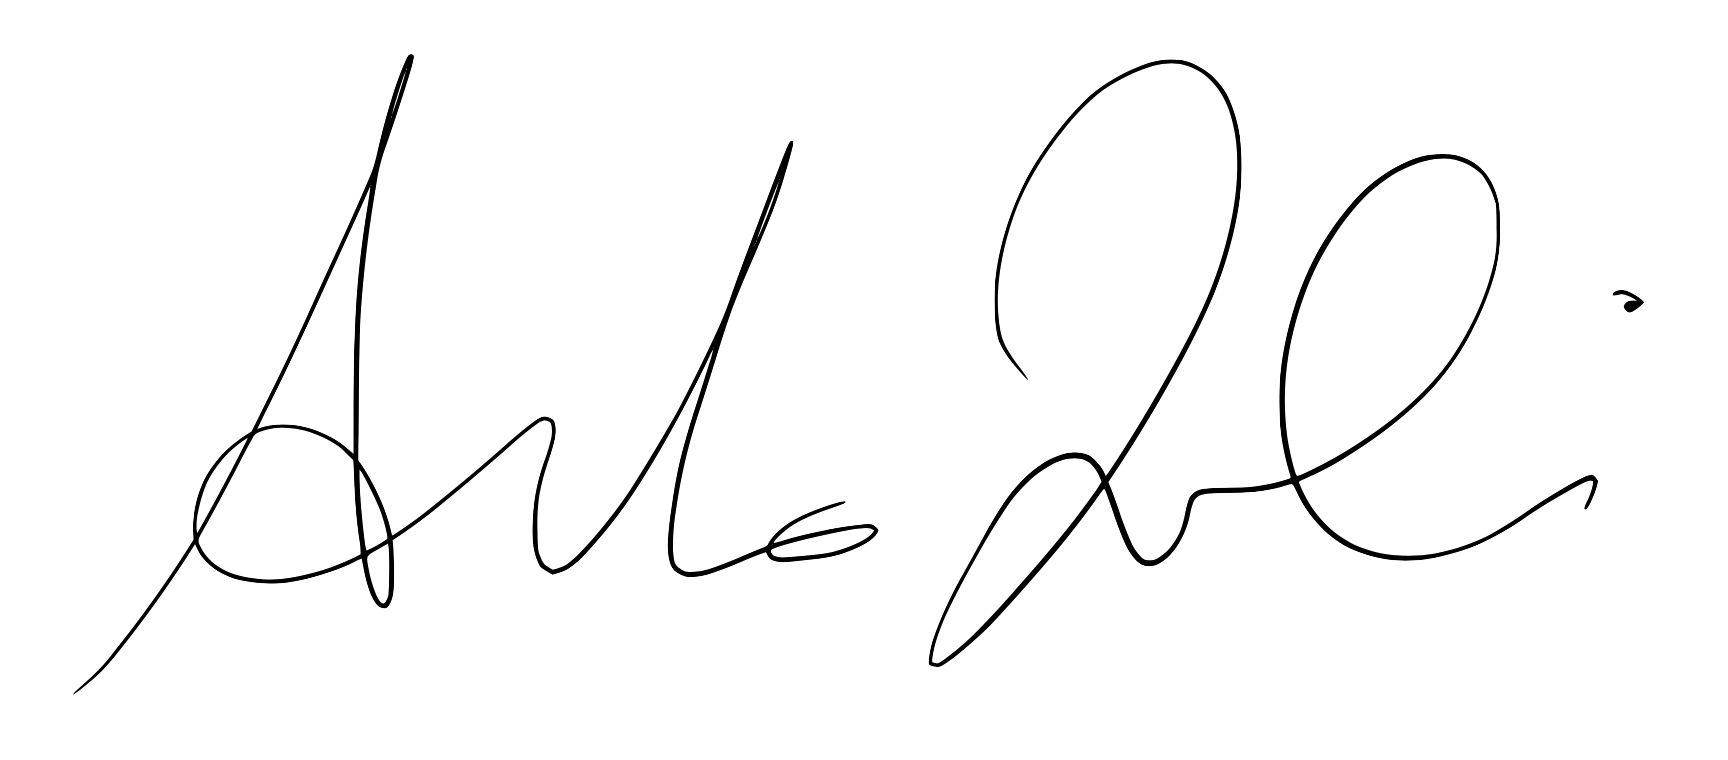
\includegraphics[width=5cm]{az_signature_transparent.png}
\end{figure}
Andrea Zignoli, February 2026
\vspace{0.5cm}
\newline
\tiny{I do hereby declare that the above given statements are true and correct to the best of my knowledge \newline
Accordingly to art. 46 and 47 of D.P.R. 445/2000} 

\end{document} 
